% Asal-usul (tidak pernah dicetak): lihat sources/outline_sources.md (Tahun 1: buku catatan
% lapangan, kompas-klinometer, kaca pembesar, pengambilan sampel, mikroskop polarisasi dan
% sayatan tipis, keselamatan). Pembacaan sayap timur antiklin Varden disimulasikan di
% figdata/bachelor-1/attitude_stats.py (seed 83, galat 3 derajat); nilai soal masalah dalam
% skrip kalkulator scratch Buku 3 calc/ch06.py.
\chapter{Metode lapangan dan laboratorium I}\label{ch:b1:field-lab-methods-1}

Seorang ahli geologi yang memetakan Perbukitan Varden hanya membawa sedikit barang: buku catatan, pensil, penerima satelit, kompas-klinometer, kaca pembesar, dan beberapa kantong sampel. Dengan itu ia menetapkan di mana ia berdiri, mengukur orientasi perlapisan, menamai batuan, dan membawa pulang sampel yang akan dipotong, digerinda, dan diamati melalui mikroskop di laboratorium. Setiap angka dalam bab-bab sebelumnya --- orientasi pada peta, \omterm{def:b1:geological-maps:attitude}{kemiringan} dalam penampang --- bermula dari pembacaan semacam ini, dengan galatnya sendiri. Bab ini menguraikan bagaimana para profesional membuat pengamatan ini, dan bagaimana pembacaan berulang dirata-ratakan serta sebarannya diubah menjadi ketidakpastian. Bab ini diakhiri dengan serangkaian pembacaan di sayap timur \omterm{def:b1:geological-maps:fold}{antiklin} Varden.

\begin{recall}
Orientasi bidang ditulis sebagai \omterm{def:b1:geological-maps:attitude}{arah kemiringan}/\omterm{def:b1:geological-maps:attitude}{kemiringan}, misalnya $081/12$, atau sebagai \omterm{def:b1:geological-maps:attitude}{jurus} menurut kaidah tangan kanan dengan \omterm{def:b1:geological-maps:attitude}{kemiringannya} (\cref{ch:b1:geological-maps}). Deklinasi magnetik adalah sudut antara utara geografis dan arah ke mana jarum kompas menunjuk (fisika, kelas 11). Mineral dikenali di tangan dari kilapnya, belahannya, kekerasannya, dan warnanya (Buku 2, kelas 11). Rata-rata dan simpangan baku suatu himpunan bilangan merangkum pusat dan sebarannya (matematika).
\end{recall}

\section{Buku catatan dan peta}

\begin{definition}[Stasiun lapangan, buku catatan lapangan]\label{def:b1:field-lab-methods-1:station}
Sebuah \emph{stasiun lapangan}\index{stasiun lapangan} adalah tempat bernomor tempat seorang ahli geologi membuat dan mencatat pengamatan: posisinya, batuan yang terlihat, orientasinya, dan sampel yang diambil. \emph{Buku catatan lapangan}\index{buku catatan lapangan} adalah catatan berjilid tentang stasiun-stasiun itu, menurut urutan kunjungannya, dengan nomornya, sketsa, dan pengukuran, yang ditulis di tempat.
\end{definition}

Buku catatan adalah catatan primer: apa yang tidak ditulis di stasiun hilang, dan peta yang digambar malam hari hanya sebaik catatan di baliknya. Setiap stasiun memiliki nomor yang muncul pada peta lapangan, di buku catatan, dan pada setiap kantong sampel yang diambil di sana. Sketsa memperlihatkan apa yang tidak dapat ditunjukkan oleh daftar angka --- bagaimana dua satuan bertemu, ke arah mana lapisan yang lebih muda berbaring, di mana pembacaan diambil pada permukaan yang terlipat --- dan mencatat skala serta orientasinya. Fakta dan interpretasi dipisahkan: ``batu gamping di atas serpih, \omterm{def:b1:geological-maps:geological-map}{kontak} tajam'' adalah pengamatan; ``\omterm{def:b1:cross-sections:unconformity}{ketidakselarasan}'' adalah inferensi, dan ditulis sebagai demikian.

\begin{inthefield}[Sehari memetakan]
% ledger: gps:smartphone-accuracy, gps:high-end
\begin{minipage}[t]{0.58\linewidth}\vspace{0pt}
Seorang ahli geologi pemetaan merencanakan lintasan melintang \omterm{def:b1:geological-maps:attitude}{jurusnya}, agar menemui setiap satuan secara bergiliran, dan berhenti di mana pun sebuah \omterm{def:b1:geological-maps:geological-map}{kontak}, perubahan batuan, atau permukaan yang dapat diukur tampak. Di setiap stasiun ia menulis nomor dan posisinya, membuat sketsa apa yang dilihatnya, mengukur orientasi, dan mencatat sampelnya. Posisi diperoleh dari penerima satelit: penerima biasa, seperti yang ada di ponsel, umumnya akurat sampai sekitar \qty{4.9}{m} di bawah langit terbuka, lebih buruk di dekat tebing dan pepohonan, sedangkan penerima survei yang memakai dua frekuensi atau layanan koreksi mencapai beberapa sentimeter. Pada skala peta 1:10\,000, \qty{4.9}{m} adalah setengah milimeter: penerima biasa cukup baik untuk pemetaan, tetapi tidak untuk mengukur gerak lambat tanah (\cref{ch:b1:plate-kinematics}).
\end{minipage}\hfill
\begin{minipage}[t]{0.39\linewidth}\vspace{0pt}
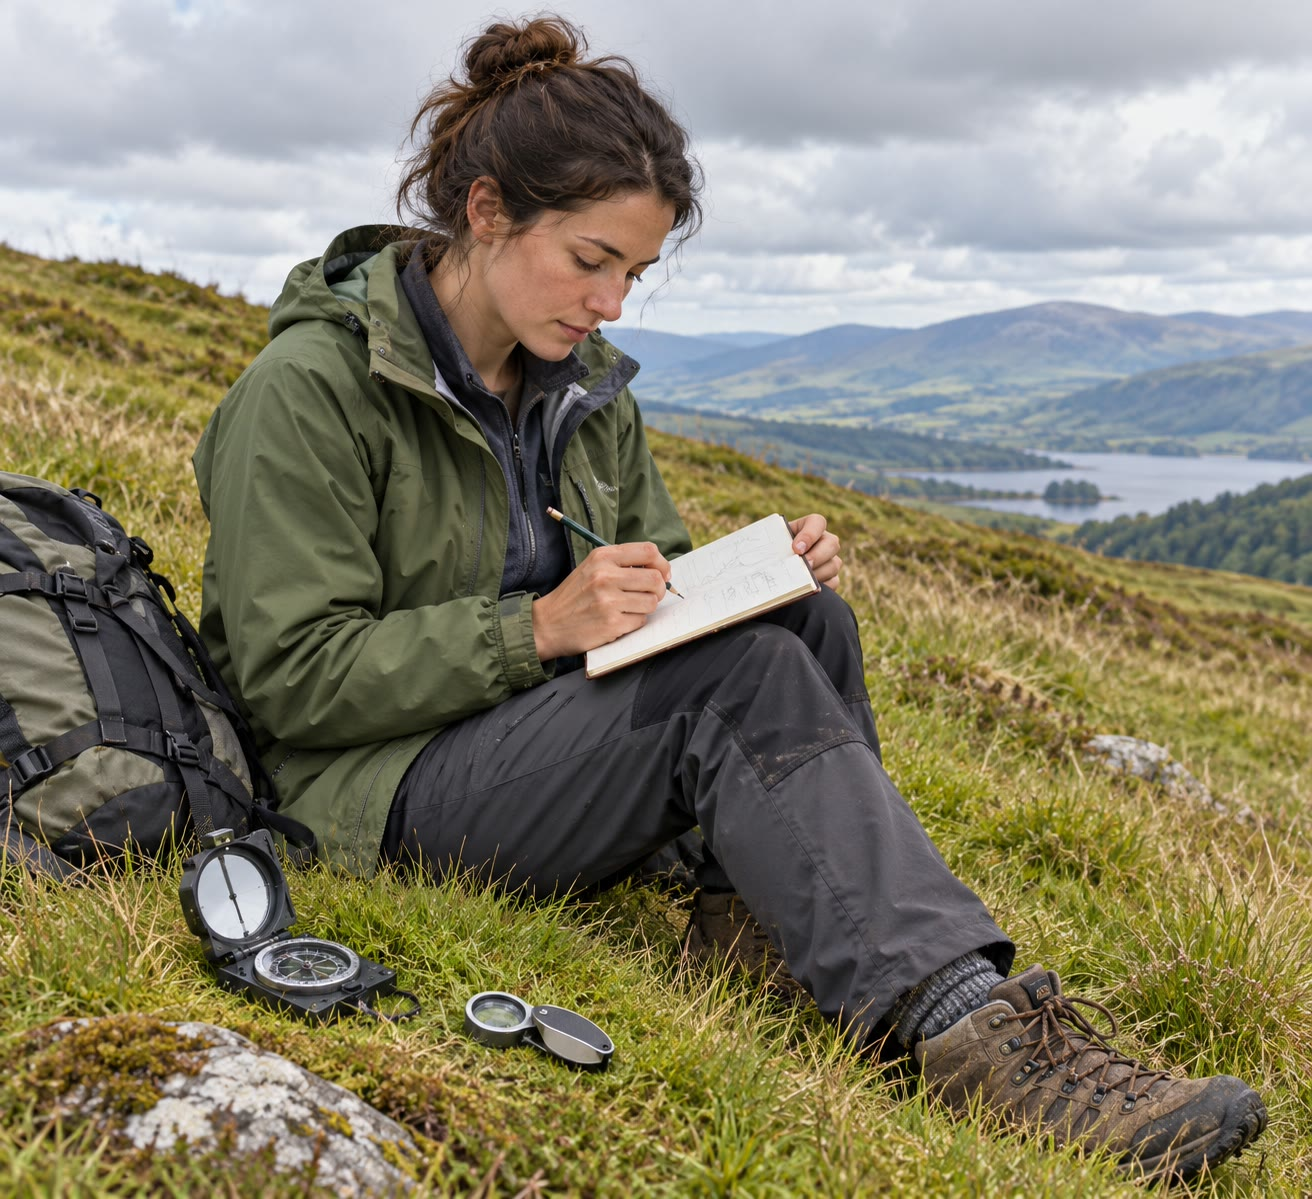
\includegraphics[width=\linewidth]{images/book3/ai/b1-field-notebook.jpg}
\end{minipage}
\end{inthefield}

\section{Mengukur orientasi}

Orientasi sebuah bidang --- perlapisan, sesar, kekar --- diukur dengan kompas-klinometer: kompas magnetik untuk membaca \omterm{def:b1:spherical-astronomy:horizontal}{azimut}, dan bandul atau nivo untuk membaca sudut dari horizontal. Tepinya diletakkan sepanjang \omterm{def:b1:geological-maps:attitude}{jurus} permukaan untuk membaca \omterm{def:b1:geological-maps:attitude}{jurus}, atau instrumen diletakkan pada permukaan sepanjang garis paling curamnya untuk membaca \omterm{def:b1:geological-maps:attitude}{kemiringan} dan, dari \omterm{def:b1:spherical-astronomy:horizontal}{azimut} garis itu, \omterm{def:b1:geological-maps:attitude}{arah kemiringan}.

\begin{omfigure}
\begin{tikzpicture}[font=\scriptsize]
% (a) plan view
\begin{scope}
\fill[icsJurassic!25] (0,0) -- (3.6,0.5) -- (3.9,2.9) -- (0.3,2.4) -- cycle;
\draw (0,0) -- (3.6,0.5) -- (3.9,2.9) -- (0.3,2.4) -- cycle;
\draw[omDef, thick] (0.4,1.55) -- (3.5,1.98);
\node[omDef, above, rotate=8, fill=icsJurassic!25, inner sep=1pt] at (0.95,1.65) {garis jurus};
% compass box laid along the strike line
\begin{scope}[shift={(2.5,1.84)}, rotate=8]
\draw[fill=white] (-0.6,0) rectangle (0.6,0.32);
\draw (0,0.16) circle (0.12);
\end{scope}
\draw[omThm, thick, -{Stealth[length=2mm]}] (1.6,1.71) -- (1.75,0.62);
\node[omThm, right, fill=icsJurassic!25, inner sep=1pt] at (1.78,0.85) {arah kemiringan};
\node[below, align=center] at (1.95,-0.15) {(a) pandangan atas: tepi kompas\\ sepanjang jurus};
\draw[->] (4.3,1.6) -- (4.3,2.4) node[above] {U};
\end{scope}
% (b) side view, vertical section along the dip direction
\begin{scope}[xshift=5.8cm]
\fill[icsJurassic!25] (0,1.6) -- (3.6,0.2) -- (3.6,-0.3) -- (0,-0.3) -- cycle;
\draw[thick] (0,1.6) -- (3.6,0.2);
% clinometer resting on the surface
\begin{scope}[shift={(2.5,0.6278)}, rotate=-21.25]
\draw[fill=white] (-0.75,0) rectangle (0.75,0.3);
\draw (0,0.15) circle (0.11);
\draw[black!70] (0,0.15) -- ++(-68.75:0.11);
\end{scope}
% dip angle at the lower end of the surface
\coordinate (P) at (0.7,1.3278);
\draw[black!60] (P) -- ++(1.6,0) node[right] {horizontal};
\draw[omThm] ($(P)+(1.1,0)$) arc[start angle=0, end angle=-21.25, radius=1.1];
\node[omThm] at ($(P)+(0.9,-0.15)$) {$\delta$};
\node[below, align=center] at (1.8,-0.35) {(b) penampang sepanjang arah kemiringan:\\ klinometer pada garis paling curam};
\end{scope}
\end{tikzpicture}

{\small Mengukur orientasi (skematis). (a) Tepi kompas yang diletakkan mendatar pada perlapisan memberikan \omterm{def:b1:geological-maps:attitude}{jurus}; \omterm{def:b1:geological-maps:attitude}{arah kemiringan} tegak lurus terhadapnya, menuruni perlapisan. (b) Diletakkan pada tepinya sepanjang garis paling curam, klinometer memberikan \omterm{def:b1:geological-maps:attitude}{kemiringan} $\delta$.}
\end{omfigure}

Sebuah garis --- \omterm{def:b1:geological-maps:fold}{sumbu lipatan}, goresan pada permukaan sesar, sumbu panjang kerikil --- memiliki orientasinya sendiri.

\begin{definition}[Trend dan penunjaman]\label{def:b1:field-lab-methods-1:trend-plunge}
\emph{Trend}\index{trend (garis)} suatu garis adalah \omterm{def:b1:spherical-astronomy:horizontal}{azimut} proyeksi horizontalnya, diukur ke arah ujung garis yang menunjuk ke bawah. \emph{Penunjaman}\index{penunjaman} adalah sudut antara garis dan horizontal, diukur dalam bidang vertikal yang memuat garis itu. Garis yang menunjam \ang{20} ke arah \ang{015} ditulis $20\to015$.
\end{definition}

Sebuah garis dengan \omterm{def:b1:field-lab-methods-1:trend-plunge}{trend} $t$ dan \omterm{def:b1:field-lab-methods-1:trend-plunge}{penunjaman} $p$ memiliki vektor satuan yang mengarah ke bawah $(\cos p\sin t, \cos p\cos t, -\sin p)$ dalam komponen timur, utara, dan atas; sebuah garis yang terletak pada bidang dengan \omterm{def:b1:geological-maps:attitude}{arah kemiringan} $\alpha$ dan \omterm{def:b1:geological-maps:attitude}{kemiringan} $\delta$ menunjam sebesar \omterm{def:b1:cross-sections:apparent-dip}{kemiringan semu} bidang itu dalam bidang vertikal berazimut $t$, sehingga $\tan p = \tan\delta\cos(\alpha - t)$ (\cref{thm:b1:cross-sections:apparent-dip}).

\subsection{Deklinasi magnetik}

Jarum kompas menunjuk ke utara magnetik, bukan utara geografis; sudut di antara keduanya adalah deklinasi magnetik, dihitung positif bila utara magnetik berada di timur utara geografis. Peta dan orientasi dalam buku ini memakai \omterm{def:b1:spherical-astronomy:horizontal}{azimut} geografis.

\begin{method}[Mengoreksi azimut kompas]\label{met:b1:field-lab-methods-1:declination}
\begin{enumerate}
  \item Carilah deklinasi magnetik $D$ untuk tempat dan tanggal itu, dari model medan Bumi (timur positif, barat negatif).
  \item Tambahkan ke setiap \omterm{def:b1:spherical-astronomy:horizontal}{azimut} yang dibaca pada kompas: \omterm{def:b1:spherical-astronomy:horizontal}{azimut} geografis $=$ \omterm{def:b1:spherical-astronomy:horizontal}{azimut} magnetik $+ D$, diambil modulo \ang{360}.
  \item Biarkan \omterm{def:b1:geological-maps:attitude}{kemiringan} dan \omterm{def:b1:field-lab-methods-1:trend-plunge}{penunjaman}: keduanya diukur dari horizontal, dengan gravitasi, bukan dengan jarum.
\end{enumerate}
Kebanyakan kompas lapangan dapat diatur untuk menambahkan $D$ secara mekanis; pengaturannya, dan tahun untuk mana ia dibuat, dicatat di buku catatan.
\end{method}

\begin{dated}{2026}
% ledger: noaa:wmm-edinburgh, noaa:wmm-reykjavik, noaa:wmm-anchorage, noaa:wmm-wellington
Pada 1 Januari 2026, Model Medan Magnet Dunia (versi 2025) memberikan deklinasi magnetik sebesar \ang{-0.47} (barat) di Edinburgh, berubah \ang{+0.20} per tahun; \ang{-11.28} di Reykjavik, berubah \ang{+0.30} per tahun; \ang{+14.20} (timur) di Anchorage, berubah \ang{-0.28} per tahun; dan \ang{+23.23} di Wellington. Seorang ahli geologi yang lupa mengoreksi di Wellington akan salah menempatkan setiap \omterm{def:b1:spherical-astronomy:horizontal}{azimut} lebih dari \ang{23}; yang memakai pengaturan Edinburgh dari sepuluh tahun sebelumnya akan membawa galat sekitar \ang{2}.
\end{dated}

\subsection{Pembacaan berulang}

Satu pembacaan pada bidang perlapisan memuat galat: permukaannya tidak pernah bidang yang sempurna, instrumennya tidak diatur sempurna, dan pembacaannya dibulatkan ke derajat. Karena itu ahli geologi mengukur permukaan yang sama beberapa kali, atau beberapa permukaan pada sayap yang sama, lalu merata-ratakan. Merata-ratakan \omterm{def:b1:spherical-astronomy:horizontal}{azimut} perlu hati-hati: pembacaan \ang{355} dan \ang{005} menggambarkan arah yang berjarak \ang{10}, tetapi rata-rata aritmetiknya, \ang{180}, menunjuk ke arah sebaliknya. Rata-rata yang benar bekerja dengan vektor.

\begin{definition}[Orientasi rata-rata (rata-rata vektor)]\label{def:b1:field-lab-methods-1:mean-orientation}
Untuk sebuah bidang dengan \omterm{def:b1:geological-maps:attitude}{arah kemiringan} $\alpha$ dan \omterm{def:b1:geological-maps:attitude}{kemiringan} $\delta$, misalkan
\[
  \vec n = (\sin\delta\sin\alpha,\ \sin\delta\cos\alpha,\ \cos\delta)
\]
adalah normal satuan ke atasnya dalam komponen timur, utara, dan atas. \emph{Orientasi rata-rata}\index{orientasi rata-rata} (atau \emph{rata-rata vektor}) dari $N$ pembacaan normal $\vec n_1, \dots, \vec n_N$ adalah bidang yang normalnya $\vec m = \vec S/\|\vec S\|$, dengan $\vec S = \sum_i \vec n_i$ adalah resultannya; $\bar R = \|\vec S\|/N$ adalah \emph{panjang resultan rata-rata}. \omterm{def:b1:geological-maps:attitude}{Arah kemiringan} dan \omterm{def:b1:geological-maps:attitude}{kemiringan} rata-rata adalah $\bar\alpha = \operatorname{atan2}(S_E, S_N)$ dan $\bar\delta = \arccos(S_U/\|\vec S\|)$.
\end{definition}

Bahwa $\vec n$ adalah normal mengikuti dari \cref{ch:b1:geological-maps}: bidang $z = -\tan\delta\,(x\sin\alpha + y\cos\alpha)$ memiliki normal ke atas $(\tan\delta\sin\alpha, \tan\delta\cos\alpha, 1)$, yang panjangnya $1/\cos\delta$.

\begin{proposition}[Rata-rata vektor adalah arah terdekat]\label{prop:b1:field-lab-methods-1:vector-mean}
Di antara semua vektor satuan $\vec u$, normal rata-rata $\vec m$ memaksimalkan
$\sum_i \vec n_i\cdot\vec u = \sum_i \cos\theta_i(\vec u)$, dengan
$\theta_i(\vec u)$ adalah sudut antara $\vec n_i$ dan $\vec u$; ekuivalennya,
ia meminimumkan $\sum_i \|\vec n_i - \vec u\|^2$. Lebih lanjut
\[
  \bar R = \frac1N\sum_i \cos\theta_i, \qquad \theta_i = \theta_i(\vec m),
\]
sehingga $0 < \bar R \le 1$, dengan $\bar R = 1$ hanya jika semua pembacaan sepakat, dan, ketika sebarannya kecil, sudut rata-rata kuadrat antara pembacaan dan rata-ratanya adalah
\[
  \theta_{\text{rms}} \approx \sqrt{2(1 - \bar R)} \quad\text{(radian)}.
\]
\end{proposition}

\begin{proof}
$\sum_i \vec n_i\cdot\vec u = \vec S\cdot\vec u \le \|\vec S\|$ menurut ketaksamaan Cauchy--Schwarz, dengan kesamaan tepat bila $\vec u = \vec m$. Karena $\|\vec n_i - \vec u\|^2 = 2 - 2\,\vec n_i\cdot\vec u$, kedua masalah itu sama. Dengan $\vec u = \vec m$ batas tercapai: $\|\vec S\| = \sum_i\cos\theta_i$, yang merupakan rumus $\bar R$. Akhirnya $\cos\theta \approx 1 - \theta^2/2$ untuk $\theta$ kecil, sehingga $1 - \bar R \approx
\frac1N\sum_i\theta_i^2/2 = \theta_{\text{rms}}^2/2$.
\end{proof}

Bagaimana galat pada kedua sudut menggerakkan normal? Dengan menurunkan $\vec n$,
\[
  \frac{\partial\vec n}{\partial\delta} = (\cos\delta\sin\alpha,\ \cos\delta\cos\alpha,\ -\sin\delta),
  \qquad
  \frac{\partial\vec n}{\partial\alpha} = (\sin\delta\cos\alpha,\ -\sin\delta\sin\alpha,\ 0):
\]
yang pertama panjangnya 1, yang kedua panjangnya $\sin\delta$, dan keduanya saling tegak lurus. Galat kecil $\Delta\delta$ dan $\Delta\alpha$ karena itu memutar normal sebesar sudut
\[
  \Delta\theta \approx \sqrt{\Delta\delta^2 + \sin^2\delta\,\Delta\alpha^2}.
\]
Pada perlapisan yang landai, galat pada \omterm{def:b1:geological-maps:attitude}{arah kemiringan} hampir tidak mengubah bidangnya: pada perlapisan yang miring \ang{12}, galat \ang{3} pada \omterm{def:b1:geological-maps:attitude}{arah kemiringan} hanya memutar bidang sebesar $3\sin\ang{12} = \ang{0.6}$. Kebalikannya adalah kesulitan ahli geologi lapangan: \omterm{def:b1:geological-maps:attitude}{arah kemiringan} perlapisan yang landai kurang tertentu oleh bidangnya, dan ketidakrataan kecil pada permukaan menyebarkannya secara lebar. Galat baku rata-rata dari $N$ pembacaan bebas dengan simpangan baku $s$ adalah $s/\sqrt N$ (matematika): untuk memangkasnya separuh, diperlukan empat kali lebih banyak pembacaan.

\begin{omfigure}
\begin{tikzpicture}
\begin{axis}[name=dd, width=0.47\linewidth, height=4.6cm, ybar, bar width=0.8,
  xmin=72.5, xmax=88.5, ymin=0, ymax=8.5, ytick={0,2,4,6,8},
  tick label style={font=\scriptsize}, label style={font=\small},
  xlabel={arah kemiringan (\si{\degree})}, ylabel={pembacaan}]
\addplot[fill=icsJurassic!40, draw=black] table[x=value, y=count] {figdata/out/bachelor-1-attitude_stats-hist-dd.dat};
\draw[omThm, thick] (axis cs:80.84,0) -- (axis cs:80.84,8.5);
\draw[omThm, densely dashed] (axis cs:77.91,0) -- (axis cs:77.91,8.5);
\draw[omThm, densely dashed] (axis cs:83.77,0) -- (axis cs:83.77,8.5);
\end{axis}
\begin{axis}[at={(dd.east)}, anchor=west, xshift=1.1cm, width=0.47\linewidth, height=4.6cm,
  ybar, bar width=0.8, xmin=5.5, xmax=18.5, ymin=0, ymax=8.5, ytick={0,2,4,6,8},
  tick label style={font=\scriptsize}, label style={font=\small},
  xlabel={kemiringan (\si{\degree})}]
\addplot[fill=icsJurassic!40, draw=black] table[x=value, y=count] {figdata/out/bachelor-1-attitude_stats-hist-dip.dat};
\draw[omThm, thick] (axis cs:12.36,0) -- (axis cs:12.36,8.5);
\draw[omThm, densely dashed] (axis cs:10.24,0) -- (axis cs:10.24,8.5);
\draw[omThm, densely dashed] (axis cs:14.48,0) -- (axis cs:14.48,8.5);
\end{axis}
\end{tikzpicture}

{\small Dua puluh lima pembacaan simulasi dari perlapisan sayap timur Varden, yang orientasi modelnya $080.7/12.2$, masing-masing dengan galat simpangan baku \ang{3} pada kedua sudut, dibulatkan ke derajat. Garis padat: rata-rata; putus-putus: satu simpangan baku di kedua sisinya ($080.8 \pm 2.9$ dan $12.4 \pm 2.1$). Rata-rata vektor dari 25 pembacaan adalah $080.9/12.3$.}
\end{omfigure}

\section{Lensa tangan dan identifikasi lapangan}

Sebagian besar batuan dinamai di lapangan, sebelum pekerjaan laboratorium, dari mineral yang ditunjukkan oleh kaca pembesar dan dari cara batuan itu pecah. Ahli geologi memandang permukaan segar, karena pelapukan melapisi dan memucatkan batuan, dan mencatat ukuran butirnya (apakah dapat dilihat dengan mata telanjang, dengan kaca pembesar, atau tidak sama sekali), bentuknya, apakah ia saling mengunci seperti mosaik atau tersemen seperti pasir, dan setiap penjajaran. Mineral dikenali dari sifat-sifat yang diingat kembali di awal bab:
kilap kaca dan tiadanya belahan pada kuarsa, dua belahan dan keputihan kusam pada feldspar, serpih mika, belahan rombohedral kalsit. Kekerasan diuji dengan ujung baja: kuarsa lebih keras daripada baja dan kalsit jauh lebih lunak.

Para profesional membawa botol tetes kecil asam klorida encer: batuan karbonat melepaskan gelembung karbon dioksida di tempat tetesan jatuh (kimia). Kalsit bereaksi cepat; dolomit bereaksi lemah kecuali bila dihaluskan. Asam ditangani dengan sarung tangan dan pelindung mata, dan tidak pernah oleh pembaca buku ini: uraian ini menggambarkan praktik profesional.

\section{Sampel}

\begin{definition}[Sampel terorientasi]\label{def:b1:field-lab-methods-1:sample}
Sebuah \emph{sampel terorientasi}\index{sampel terorientasi} adalah sampel batuan tempat ahli geologi telah menandai, sebelum mengambilnya, orientasi salah satu permukaannya (garis \omterm{def:b1:geological-maps:attitude}{jurus} dan panah \omterm{def:b1:geological-maps:attitude}{kemiringan}, atau \omterm{def:b1:field-lab-methods-1:trend-plunge}{trend} suatu garis), sehingga sampel itu dapat dikembalikan ke posisi lapangannya di laboratorium.
\end{definition}

Sampel hanya berguna bila ia mewakili satuan yang diwakilinya --- segar, tidak lapuk, tidak diambil dari urat atau balok yang jatuh --- dan bila asalnya pasti. Setiap sampel menerima nomor stasiun dan nomor sampel, yang ditulis pada batuannya dan pada kantongnya, serta dicantumkan di buku catatan dengan posisinya, satuannya, dan alasan pengambilannya. Sampel untuk analisis kimia atau isotop, yang hasilnya mungkin diterbitkan puluhan tahun kemudian, dilacak dari lapangan ke laboratorium dengan catatan tertulis tentang setiap tangan yang dilaluinya --- rantai penyimpanan --- sehingga tidak ada keraguan tentang batuan mana yang memberi nomor mana. \omterm{def:b1:field-lab-methods-1:sample}{Sampel terorientasi} diperlukan setiap kali arah sesuatu di dalam batuan penting: penjajaran mineral, fabrik yang terlihat di bawah mikroskop, atau arah magnetisasi yang diperoleh batuan ketika ia terbentuk.

\section{Sayatan tipis dan mikroskop polarisasi}

\begin{definition}[Sayatan tipis]\label{def:b1:field-lab-methods-1:thin-section}
Sebuah \emph{sayatan tipis}\index{sayatan tipis} adalah irisan batuan, yang direkatkan pada kaca objek dan digerinda hingga ketebalan baku \qty{30}{\micro\metre}, cukup tipis agar sebagian besar mineral meneruskan cahaya.
\end{definition}

\begin{inthelab}[Membuat sayatan tipis]
% ledger: jaic:thin-section, jaic:epoxy-ri
\begin{minipage}[t]{0.58\linewidth}\vspace{0pt}
Di laboratorium persiapan, seorang teknisi memotong sebuah balok kecil dari sampel dengan gergaji intan, menggerinda satu permukaannya hingga benar-benar rata, dan merekatkannya pada kaca objek dengan resin epoksi yang indeks biasnya, 1.54 hingga 1.55, hampir sama dengan kuarsa. Sebagian besar balok itu kemudian digergaji, dan irisannya digerinda pada piringan berputar dengan abrasif yang makin halus hingga tebalnya \qty{30}{\micro\metre}. Teknisi memeriksa ketebalannya di bawah mikroskop dari warna yang diperlihatkan butir kuarsa (\cref{ch:b1:optical-mineralogy}), dan menyelesaikannya dengan kaca penutup tipis atau permukaan yang dipoles. Batuan yang berpori atau rapuh lebih dahulu direndam dalam resin agar tetap utuh.
\end{minipage}\hfill
\begin{minipage}[t]{0.39\linewidth}\vspace{0pt}
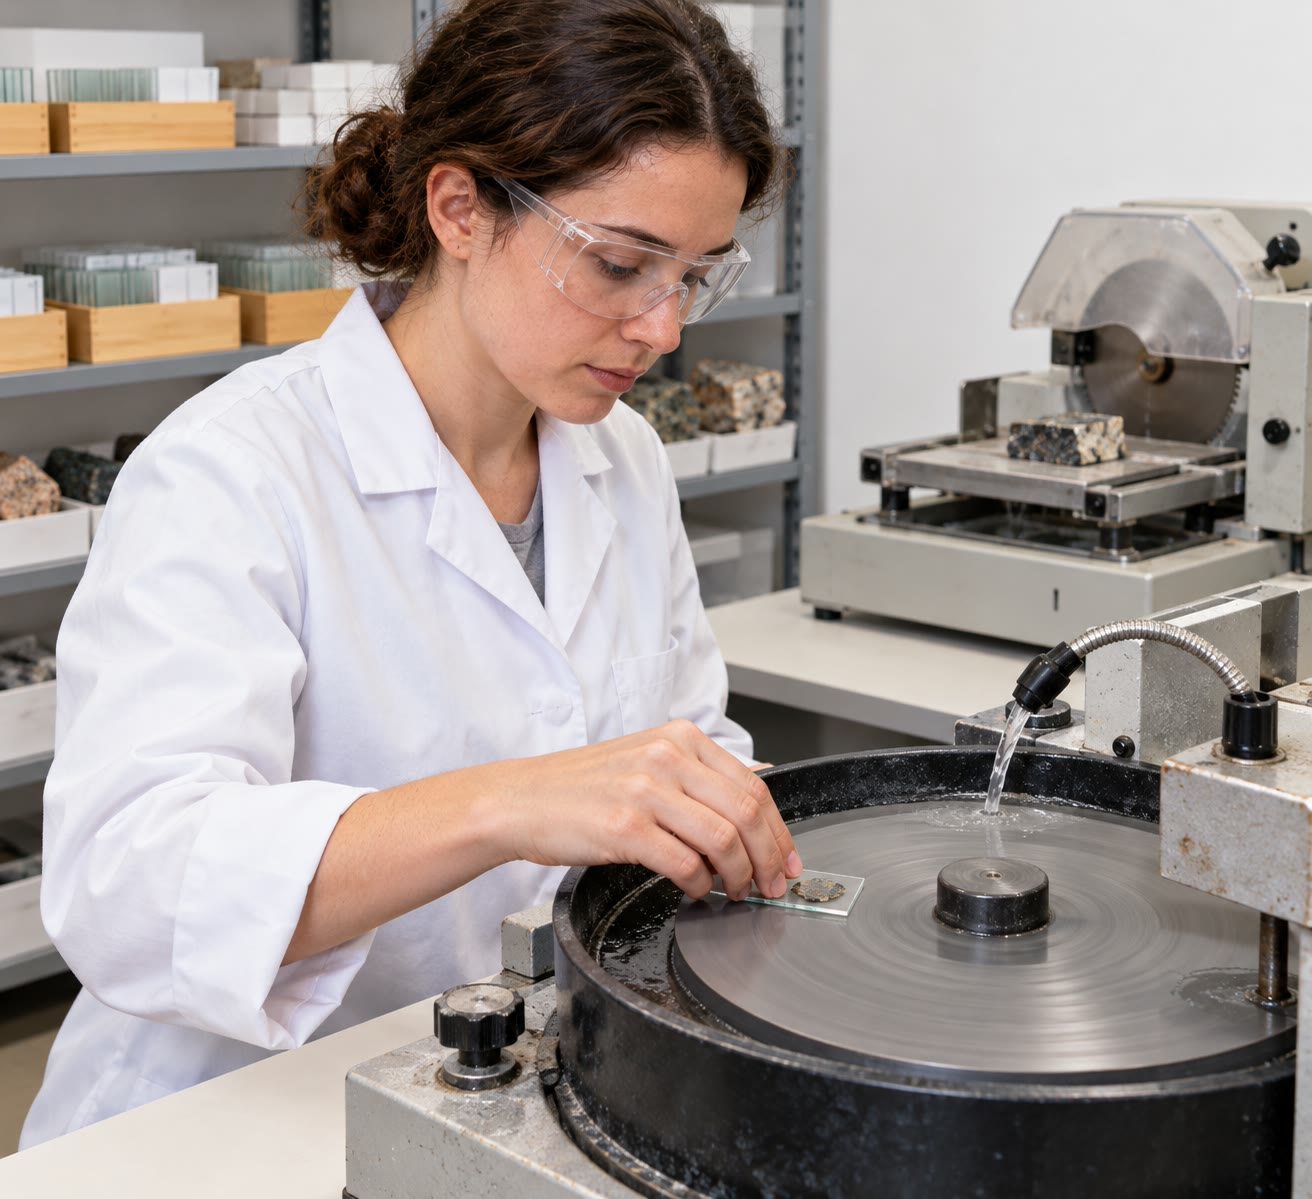
\includegraphics[width=\linewidth]{images/book3/ai/b1-thin-section-lab.jpg}
\end{minipage}
\end{inthelab}

\omterm{def:b1:field-lab-methods-1:thin-section}{Sayatan tipis} diamati dengan mikroskop yang dilengkapi dua filter polarisasi. Polarisasi linear adalah pokok bahasan fisika: di sini cukup bahwa filter polarisasi hanya meneruskan cahaya yang bergetar pada satu arah, dan bahwa dua filter yang diatur tegak lurus tidak meneruskan apa pun.

\begin{definition}[Mikroskop polarisasi, cahaya terpolarisasi bidang, polarisasi silang]\label{def:b1:field-lab-methods-1:microscope}
Sebuah \emph{mikroskop polarisasi}\index{mikroskop polarisasi} adalah mikroskop cahaya yang diteruskan dengan filter polarisasi (polarisator) di bawah meja yang berputar sepanjang \ang{360} terhadap skala berderajat, dan filter polarisasi kedua (analisator) di antara objektif dan okuler, yang dapat digerakkan masuk atau keluar dari jalur cahaya, dengan arah getarnya tegak lurus terhadap arah polarisator. Dengan analisator keluar, spesimen terlihat dalam \emph{cahaya terpolarisasi bidang}\index{cahaya terpolarisasi bidang}; dengan analisator masuk, ia terlihat di antara \emph{polarisasi silang}\index{polarisasi silang}.
\end{definition}

\begin{omfigure}
\begin{tikzpicture}[font=\scriptsize, x=1cm, y=0.62cm]
\def\comp#1#2#3{\draw[fill=#3] (-1.1,#1-0.18) rectangle (1.1,#1+0.18); \node[right] at (1.3,#1) {#2};}
\draw[omThm!60, line width=3pt, -{Stealth[length=3mm]}] (0,0.3) -- (0,10.6);
\draw[fill=yellow!40] (0,0) circle (0.3); \node[right] at (1.3,0) {lampu};
\comp{1.3}{polarisator: meneruskan satu arah getar}{omDef!25}
\draw[omDef, thick, <->] (-0.5,1.3) -- (0.5,1.3);
\draw[fill=white] (-1.0,2.3) .. controls (0,2.75) .. (1.0,2.3) .. controls (0,1.85) .. (-1.0,2.3);
\node[right] at (1.3,2.3) {kondensor};
\draw[fill=black!70] (-1.6,3.4) rectangle (1.6,3.55);
\draw[fill=icsJurassic!40] (-0.5,3.55) rectangle (0.5,3.65);
\node[right] at (1.7,3.48) {meja putar, berskala derajat, dengan sayatan tipis};
\draw[fill=white] (-0.45,4.5) rectangle (0.45,5.4); \node[right] at (1.3,4.95) {objektif};
\comp{6.2}{celah aksesori}{black!10}
\comp{7.2}{analisator: masuk (polarisasi silang) atau keluar (cahaya terpolarisasi bidang)}{omDef!25}
\draw[omDef, thick, <->] (0,6.85) -- (0,7.55);
\comp{8.2}{lensa Bertrand (opsional)}{black!5}
\draw[fill=white] (-0.35,9.1) rectangle (0.35,10.0); \node[right] at (1.3,9.55) {okuler dengan kisi silang};
\end{tikzpicture}

{\small Jalur cahaya \omterm{def:b1:field-lab-methods-1:microscope}{mikroskop polarisasi} (skematis, dari bawah ke atas). Polarisator dan analisator bergetar tegak lurus (panah ganda); tanpa apa pun di antaranya, \omterm{def:b1:field-lab-methods-1:microscope}{polarisasi silang} memberi medan hitam.}
\end{omfigure}

Di antara \omterm{def:b1:field-lab-methods-1:microscope}{polarisasi silang}, kaca objek, epoksi, dan mineral isotropik apa pun (yang sifat optiknya sama di setiap arah, seperti pada kristal kubik) tetap hitam apa pun putaran mejanya. Sebagian besar mineral tidak isotropik: mereka mengubah polarisasi cahaya yang melewatinya, dan tampak dalam warna interferensi yang berubah ketika meja berputar serta menghilang empat kali dalam satu putaran penuh. Mengapa demikian, dan bagaimana warna serta sudut itu mengidentifikasi suatu mineral, adalah pokok bahasan \cref{ch:b1:optical-mineralogy}. Mineral dalam \omterm{def:b1:field-lab-methods-1:thin-section}{sayatan tipis} biasanya diamati pada pembesaran sekitar $16\times$ sampai $400\times$.
% ledger: jaic:magnification

\begin{omfigure}
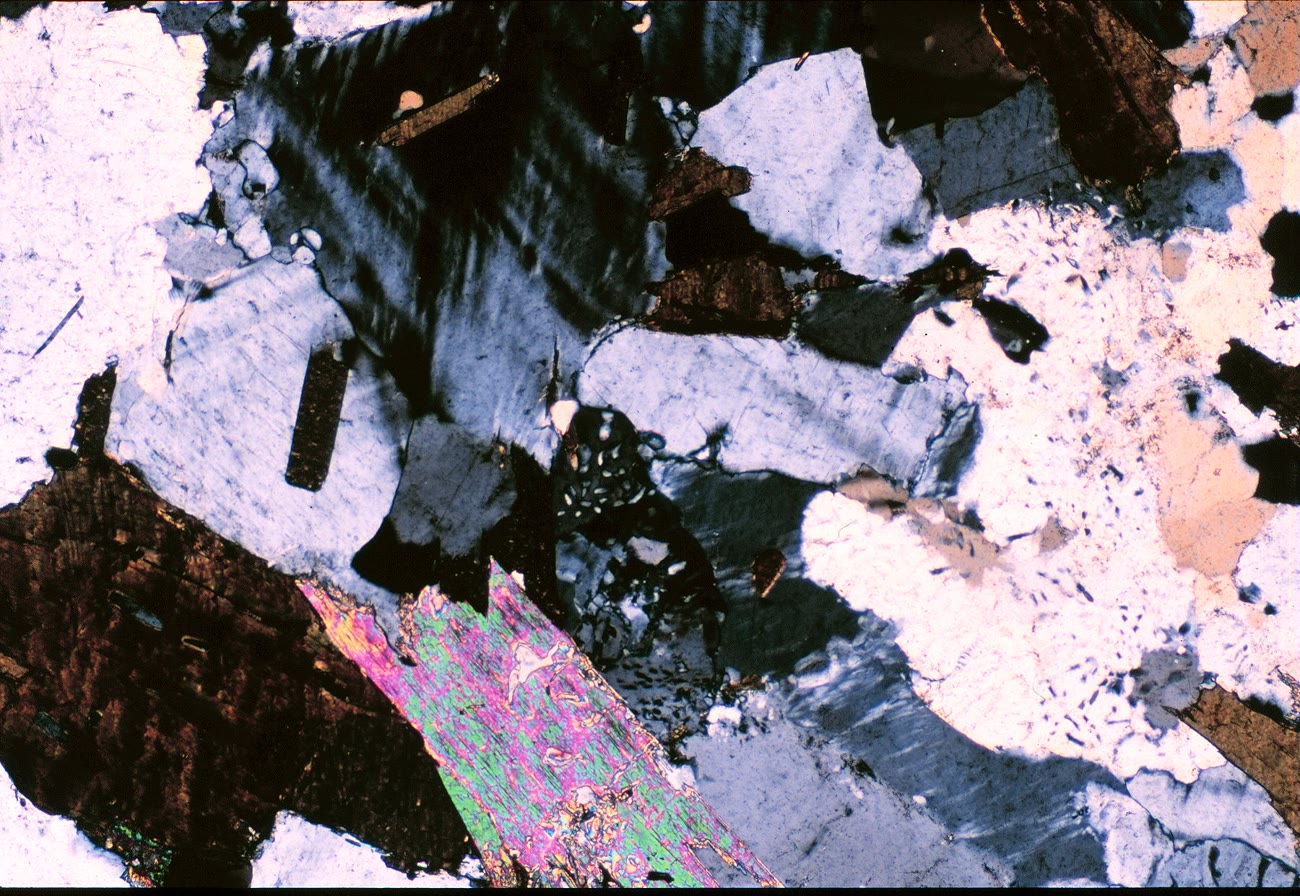
\includegraphics[width=0.55\linewidth]{images/book3/b1-granite-thin-section-xpl.jpg}
% ledger: commons:granite-xpl

{\small Granit dalam \omterm{def:b1:field-lab-methods-1:thin-section}{sayatan tipis} di antara \omterm{def:b1:field-lab-methods-1:microscope}{polarisasi silang}. Biotit berwarna cokelat, muskovit memperlihatkan warna interferensi merah muda dan hijau yang cerah, plagioklas bergaris oleh kembarannya, dan kuarsa putih hingga kelabu. Foto Darla Sondrol, CC0 (Wikimedia Commons).}
\end{omfigure}

\begin{safety}
Kerja lapangan dan laboratorium dibuat aman oleh aturan profesional, bukan oleh keberuntungan. Di lapangan, ahli geologi bekerja berpasangan atau meninggalkan rencana tertulis tentang rute dan waktu kembalinya; mereka membawa prakiraan cuaca, peta, dan pertolongan pertama, menjauh dari kaki dan tepi tebing serta muka kuari, dan memakai helm serta pelindung mata di mana pun batuan dapat jatuh atau pecah; kerja di lokasi aktif mengikuti aturan pengelolanya. Di laboratorium, gergaji dan piringan bekerja di balik pelindung dengan air untuk menekan debu, resin dan asam ditangani dengan sarung tangan dan kacamata di bawah pengisapan, dan setiap bahan kimia memiliki lembar data keselamatannya. Tidak satu pun kegiatan ini ditujukan untuk pembaca buku ini saja: bab ini menguraikan praktik profesional.
\end{safety}

\section{Latihan}

\begin{exercise}[$\star$]\label{exo:b1:field-lab-methods-1:1}
Sebuah penerima satelit memberikan posisi dalam sekitar \qty{4.9}{m}. Seberapa besar itu pada peta 1:10\,000? Pada 1:25\,000?
\end{exercise}

\begin{exercise}[$\star$]\label{exo:b1:field-lab-methods-1:2}
Sebuah kompas tanpa pengaturan deklinasi membaca \omterm{def:b1:geological-maps:attitude}{arah kemiringan} \ang{052} pada suatu perlapisan. Berikan \omterm{def:b1:geological-maps:attitude}{arah kemiringan} geografisnya bila pembacaan dibuat di Reykjavik pada 1 Januari 2026, lalu di Wellington pada hari yang sama (kotak bertanggal).
\end{exercise}

\begin{exercise}[$\star$]\label{exo:b1:field-lab-methods-1:3}
Sebuah \omterm{def:b1:geological-maps:fold}{sumbu lipatan} menunjam \ang{20} ke arah \ang{015}. Tuliskan orientasinya seperti dalam teks dan berikan vektor satuan ke bawahnya dalam komponen timur, utara, dan atas.
\end{exercise}

\begin{exercise}[$\star$]\label{exo:b1:field-lab-methods-1:4}
Tiga pembacaan sebuah kekar vertikal memberikan \omterm{def:b1:spherical-astronomy:horizontal}{azimut} normalnya \ang{350}, \ang{358} dan \ang{006}. Hitunglah rata-rata aritmetiknya, lalu \omterm{def:b1:spherical-astronomy:horizontal}{azimut} jumlah ketiga vektor satuan horizontalnya. Rata-rata mana yang benar?
\end{exercise}

\begin{exercise}[$\star\star$]\label{exo:b1:field-lab-methods-1:5}
Lima pembacaan \omterm{def:b1:geological-maps:attitude}{kemiringan} satu perlapisan adalah \ang{34}, \ang{37}, \ang{35}, \ang{33} dan \ang{36}. Hitunglah rata-ratanya, simpangan bakunya, dan galat baku rata-ratanya.
\end{exercise}

\begin{exercise}[$\star\star$]\label{exo:b1:field-lab-methods-1:6}
Seorang ahli geologi merata-ratakan satu pembacaan pada tiap sayap \omterm{def:b1:geological-maps:fold}{lipatan} simetris: $090/30$ dan $270/30$. Hitunglah rata-rata vektor dan $\bar R$. Apa yang salah?
\end{exercise}

\begin{exercise}[$\star\star$]\label{exo:b1:field-lab-methods-1:7}
Goresan pada permukaan perlapisan berorientasi $080/12$ memiliki \omterm{def:b1:field-lab-methods-1:trend-plunge}{trend} \ang{120}. Berapakah \omterm{def:b1:field-lab-methods-1:trend-plunge}{penunjamannya}? Berapakah bila \omterm{def:b1:field-lab-methods-1:trend-plunge}{trend-nya} \ang{170}?
\end{exercise}

\begin{exercise}[$\star\star$]\label{exo:b1:field-lab-methods-1:8}
Di Edinburgh deklinasi magnetik adalah \ang{-0.47} pada 1 Januari 2026 dan berubah \ang{+0.20} per tahun. Dengan asumsi perubahannya tetap, kapan ia mencapai nol, dan berapakah nilainya pada 1 Januari 2030?
\end{exercise}

\begin{exercise}[$\star\star$]\label{exo:b1:field-lab-methods-1:9}
Tiga pembacaan satu perlapisan adalah $080/10$, $080/12$ dan $080/14$. Tunjukkan bahwa rata-rata vektornya adalah $080/12$, hitunglah $\bar R$ dan taksiran $\sqrt{2(1 - \bar R)}$ dari $\theta_{\text{rms}}$, dan bandingkan dengan sudut akar rata-rata kuadrat yang eksak.
\end{exercise}

\begin{exercise}[$\star\star\star$]\label{exo:b1:field-lab-methods-1:10}
Sebuah \omterm{def:b1:field-lab-methods-1:thin-section}{sayatan tipis} memotong butir bola berjari-jari $r$ pada jarak $h$ dari pusatnya, dengan $h$ sama mungkin di mana saja antara 0 dan $r$. Tunjukkan bahwa jari-jari rata-rata lingkaran yang terlihat dalam sayatan adalah $\pi r/4$. Butir kuarsa selebar \qty{0.50}{mm} rata-rata tampak seberapa besar dalam \omterm{def:b1:field-lab-methods-1:thin-section}{sayatan tipis}?
\end{exercise}

\begin{exercise}[$\star\star\star$]\label{exo:b1:field-lab-methods-1:11}
Tunjukkan bahwa bila setiap \omterm{def:b1:geological-maps:attitude}{arah kemiringan} dari suatu himpunan pembacaan ditambah dengan sudut yang sama $D$, \omterm{def:b1:geological-maps:attitude}{arah kemiringan} rata-rata vektornya bertambah $D$ dan \omterm{def:b1:geological-maps:attitude}{kemiringannya} tidak berubah. Mengapa ini penting bagi koreksi deklinasi?
\end{exercise}

\begin{exercise}[$\star\star\star$]\label{exo:b1:field-lab-methods-1:12}
Pada perlapisan yang miring \ang{12}, normal satu pembacaan tersebar dengan simpangan baku \ang{2} pada masing-masing dua arah yang saling tegak lurus: sepanjang garis \omterm{def:b1:geological-maps:attitude}{kemiringan} paling curam, yang mengubah \omterm{def:b1:geological-maps:attitude}{kemiringan}, dan melintangnya, yang mengubah \omterm{def:b1:geological-maps:attitude}{arah kemiringan}. Berapa pembacaan yang diperlukan agar galat baku \omterm{def:b1:geological-maps:attitude}{kemiringan} rata-rata \ang{0.5}? Agar \omterm{def:b1:geological-maps:attitude}{arah kemiringan} rata-rata \ang{1}?
\end{exercise}

\section{Soal: Musim lapangan di sayap timur Varden}

\begin{problem}[{Soal akhir pekan --- merata-ratakan dua belas pembacaan kompas, mengukur sebarannya, mengoreksinya, dan membandingkannya dengan lubang bor}]
\label{pb:b1:field-lab-methods-1:1}
% readings: figdata/bachelor-1/attitude_stats.py (part normals); values: calc/ch06.py
Seorang ahli geologi mengukur perlapisan sayap timur \omterm{def:b1:geological-maps:fold}{antiklin} Varden di dua belas stasiun, dengan kompas yang diatur untuk deklinasi, dan membulatkan ke derajat. Tabel memberikan setiap pembacaan (\omterm{def:b1:geological-maps:attitude}{arah kemiringan}/\omterm{def:b1:geological-maps:attitude}{kemiringan}) dan komponen normal satuan ke atasnya $\vec n = (n_E, n_N, n_U)$, dibulatkan ke empat desimal.
\begin{center}
\small
\begin{tabular}{rcccc@{\qquad}rcccc}
\hline
 & pembacaan & $n_E$ & $n_N$ & $n_U$ & & pembacaan & $n_E$ & $n_N$ & $n_U$ \\
\hline
1 & $076/11$ & 0.1851 & 0.0462 & 0.9816 & 7 & $083/11$ & 0.1894 & 0.0233 & 0.9816 \\
2 & $081/13$ & 0.2222 & 0.0352 & 0.9744 & 8 & $083/12$ & 0.2064 & 0.0253 & 0.9781 \\
3 & $078/16$ & 0.2696 & 0.0573 & 0.9613 & 9 & $085/12$ & 0.2071 & 0.0181 & 0.9781 \\
4 & $081/11$ & 0.1885 & 0.0298 & 0.9816 & 10 & $078/11$ & 0.1866 & 0.0397 & 0.9816 \\
5 & $076/10$ & 0.1685 & 0.0420 & 0.9848 & 11 & $081/13$ & & & \\
6 & $083/14$ & 0.2401 & 0.0295 & 0.9703 & 12 & $082/11$ & & & \\
\hline
\end{tabular}
\end{center}

\medskip
\noindent\textbf{Bagian I --- Orientasi rata-rata.}
\begin{enumerate}
  \item Hitunglah rata-rata aritmetik dari dua belas \omterm{def:b1:geological-maps:attitude}{arah kemiringan} dan dari dua belas \omterm{def:b1:geological-maps:attitude}{kemiringan}.
  \item Berikan contoh dua pembacaan yang rata-rata aritmetik \omterm{def:b1:geological-maps:attitude}{arah kemiringannya} tidak masuk akal, dan jelaskan mengapa di sini aman.
  \item Tunjukkan bahwa $\vec n = (\sin\delta\sin\alpha, \sin\delta\cos\alpha,
        \cos\delta)$ adalah vektor satuan yang tegak lurus pada garis \omterm{def:b1:geological-maps:attitude}{kemiringan} dan pada garis \omterm{def:b1:geological-maps:attitude}{jurus} bidang $\alpha/\delta$.
  \item Lengkapi tabel untuk pembacaan 11 dan 12.
  \item Hitunglah resultan $\vec S$ dari dua belas normal.
  \item Hitunglah $\|\vec S\|$ dan panjang resultan rata-rata $\bar R$.
  \item Turunkan rata-rata vektornya: \omterm{def:b1:geological-maps:attitude}{arah kemiringan} dan \omterm{def:b1:geological-maps:attitude}{kemiringannya}.
\end{enumerate}

\medskip
\noindent\textbf{Bagian II --- Sebaran.}
\begin{enumerate}[resume]
  \item Hitunglah simpangan baku sampel dari \omterm{def:b1:geological-maps:attitude}{arah kemiringan} dan dari \omterm{def:b1:geological-maps:attitude}{kemiringan}.
  \item Dengan memakai \cref{prop:b1:field-lab-methods-1:vector-mean}, taksirkan sudut akar rata-rata kuadrat $\theta_{\text{rms}}$ antara pembacaan dan rata-ratanya, dalam derajat.
  \item Prediksikan $\theta_{\text{rms}}$ dari kedua simpangan baku soal 8 dan rumus galat dalam bab ini, lalu bandingkan.
  \item Di antara kedua simpangan baku, mana yang paling banyak berkontribusi pada $\theta_{\text{rms}}$, dan mengapa?
  \item Hitunglah galat baku \omterm{def:b1:geological-maps:attitude}{kemiringan} rata-rata dan \omterm{def:b1:geological-maps:attitude}{arah kemiringan} rata-rata.
  \item Apakah sebaran \omterm{def:b1:geological-maps:attitude}{arah kemiringan}, \ang{2.9}, merupakan tanda pengukuran yang ceroboh? Jelaskan.
\end{enumerate}

\medskip
\noindent\textbf{Bagian III --- Deklinasi.}
\begin{enumerate}[resume]
  \item Seorang ahli geologi kedua lupa mengatur deklinasi. Dua belas pembacaannya memiliki rata-rata vektor $083.1/12.1$ dalam \omterm{def:b1:spherical-astronomy:horizontal}{azimut} magnetik. Anggaplah deklinasi magnetik di Perbukitan Varden tahun itu adalah \ang{2.5} barat. Berapakah rata-ratanya dalam \omterm{def:b1:spherical-astronomy:horizontal}{azimut} geografis?
  \item Mengapa \omterm{def:b1:geological-maps:attitude}{kemiringan} rata-ratanya benar tanpa koreksi?
  \item Dapatkah ia mengoreksi setiap pembacaan sebelum merata-ratakan, bukan rata-ratanya? Apakah itu mengubah jawabannya (\cref{exo:b1:field-lab-methods-1:11})?
  \item Sepuluh tahun kemudian, seorang mahasiswa memakai kembali pengaturan deklinasinya sementara deklinasinya telah berubah \ang{0.2} per tahun. Berapa besar galatnya, dibandingkan dengan galat baku soal 12?
  \item Berikan \omterm{def:b1:geological-maps:attitude}{jurus} \omterm{def:b1:field-lab-methods-1:mean-orientation}{orientasi rata-rata} ahli geologi pertama menurut kaidah tangan kanan.
\end{enumerate}

\medskip
\noindent\textbf{Bagian IV --- Kompas dan lubang bor.}
\begin{enumerate}[resume]
  \item Dari tiga lubang bor, \cref{ch:b1:geological-maps} memperoleh orientasi $080.6/12.2$ untuk dasar batu gamping. Bandingkan dengan rata-rata vektor soal 7, sudut demi sudut.
  \item Hitunglah sudut antara kedua normal.
  \item Galat baku arah rata-rata kira-kira $\theta_{\text{rms}}/\sqrt N$. Apakah selisih soal 20 bermakna?
  \item Berapa pembacaan yang akan memangkas galat baku itu separuh?
  \item Sebutkan dua galat yang tidak akan dikurangi oleh berapa pun jumlah pembacaan.
  \item Berikan \omterm{def:b1:field-lab-methods-1:mean-orientation}{orientasi rata-rata} sayap timur dari dua belas pembacaan, dalam bentuk \omterm{def:b1:geological-maps:attitude}{arah kemiringan}/\omterm{def:b1:geological-maps:attitude}{kemiringan} yang dibulatkan ke derajat.
\end{enumerate}
\end{problem}
